\newpage\subsection*{Άσκηση 1}

Σε ένα μΥ-Σ $8085$ να γραφεί σε \en{assembly} το παρακάτω πρόγραμμα που δίνεται σε γλώσσα μηχανής και να εξηγηθεί η
λειτουργία του:

\selectlanguage{english}
\begin{center}
    \textbf{0E} 08 \textbf{3A} 00 20 \textbf{17} \textbf{DA} 0D 08 \textbf{0D} \textbf{C2} 05 08 \textbf{79} \textbf{2F} \textbf{32} 00 30 \textbf{CF}
\end{center}
\selectlanguage{greek}

Το πρόγραμμα υποθέτουμε ότι είναι φορτωμένο στη μνήμη με αρχή τη διεύθυνση 0800 και δίνεται για διευκόλυνσή σας ότι
οι \en{bold} κωδικοί είναι εντολές.

\subsubsection*{Λύση}

Παρατίθεται το πρόγραμμα τροποποιημένο για να λειτουργεί με τον \en{simulator}:

\selectlanguage{english}
    \inputminted{text}{askisi1.8085}
\selectlanguage{greek}

Καθώς επίσης και το \en{flow graph}:


\begin{center}
    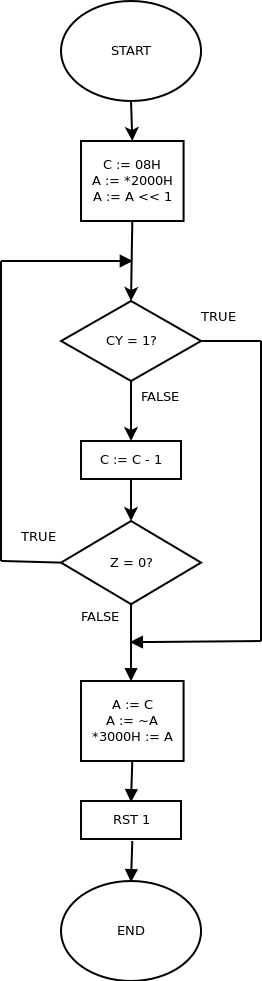
\includegraphics[width=3cm, height=10cm, center]{Diagram1.png}
\end{center}


Το παραπάνω πρόγραμμα παίρνει την είσοδο μέσω των \en{dip switch}, υπολογίζει τη θέση του πρώτου απο τα αριστερά \en{bit}
που είναι 1 και μας τον δίνει σε δυαδική μορφή μέσω των \en{led}.
